
\documentclass[journal,12pt,twocolumn]{IEEEtran}
%
\usepackage{setspace}
\usepackage{gensymb}
\singlespacing
\usepackage[cmex10]{amsmath}
\usepackage{siunitx}
\usepackage{amsthm}

\usepackage{mathrsfs}

\usepackage{txfonts}
\usepackage{stfloats}

\usepackage{steinmetz}
\usepackage{cite}
\usepackage{cases}
\usepackage{subfig}
\usepackage{longtable}
\usepackage{multirow}
\usepackage{enumitem}
\usepackage{mathtools}
\usepackage{tikz}
\usepackage{circuitikz}
\usepackage{verbatim}
\usepackage{tfrupee}
\usepackage[breaklinks=true]{hyperref}
\usepackage{tkz-euclide} % loads  TikZ and tkz-base
\usetikzlibrary{calc,math}
\usetikzlibrary{fadings}
\usepackage{listings}
    \usepackage{color}                                            %%
    \usepackage{array}                                            %%
    \usepackage{longtable}                                        %%
    \usepackage{calc}                                             %%
    \usepackage{multirow}                                         %%
    \usepackage{hhline}                                           %%
    \usepackage{ifthen}                                           %%
  %optionally (for landscape tables embedded in another document): %%
    \usepackage{lscape}     
\usepackage{multicol}
\usepackage{chngcntr}
\DeclareMathOperator*{\Res}{Res}

\renewcommand\thesection{\arabic{section}}
\renewcommand\thesubsection{\thesection.\arabic{subsection}}
\renewcommand\thesubsubsection{\thesubsection.\arabic{subsubsection}}

\renewcommand\thesectiondis{\arabic{section}}
\renewcommand\thesubsectiondis{\thesectiondis.\arabic{subsection}}
\renewcommand\thesubsubsectiondis{\thesubsectiondis.\arabic{subsubsection}}

\hyphenation{op-tical net-works semi-conduc-tor}
\def\inputGnumericTable{}                                 %%

\lstset{
%language=C,
frame=single, 
breaklines=true,
columns=fullflexible
}
\begin{document}
%


\newtheorem{theorem}{Theorem}[section]
\newtheorem{problem}{Problem}
\newtheorem{proposition}{Proposition}[section]
\newtheorem{lemma}{Lemma}[section]
\newtheorem{corollary}[theorem]{Corollary}
\newtheorem{example}{Example}[section]
\newtheorem{definition}[problem]{Definition}
\newcommand{\BEQA}{\begin{eqnarray}}
\newcommand{\EEQA}{\end{eqnarray}}
\newcommand{\define}{\stackrel{\triangle}{=}}
\bibliographystyle{IEEEtran}
\providecommand{\mbf}{\mathbf}
\providecommand{\pr}[1]{\ensuremath{\Pr\left(#1\right)}}
\providecommand{\qfunc}[1]{\ensuremath{Q\left(#1\right)}}
\providecommand{\sbrak}[1]{\ensuremath{{}\left[#1\right]}}
\providecommand{\lsbrak}[1]{\ensuremath{{}\left[#1\right.}}
\providecommand{\rsbrak}[1]{\ensuremath{{}\left.#1\right]}}
\providecommand{\brak}[1]{\ensuremath{\left(#1\right)}}
\providecommand{\lbrak}[1]{\ensuremath{\left(#1\right.}}
\providecommand{\rbrak}[1]{\ensuremath{\left.#1\right)}}
\providecommand{\cbrak}[1]{\ensuremath{\left\{#1\right\}}}
\providecommand{\lcbrak}[1]{\ensuremath{\left\{#1\right.}}
\providecommand{\rcbrak}[1]{\ensuremath{\left.#1\right\}}}
\theoremstyle{remark}
\newtheorem{rem}{Remark}
\newcommand{\sgn}{\mathop{\mathrm{sgn}}}
\providecommand{\abs}[1]{\left\vert#1\right\vert}
\providecommand{\abs}[1]{\lvert#1\rvert} 
\providecommand{\res}[1]{\Res\displaylimits_{#1}} 
\providecommand{\norm}[1]{\left\lVert#1\right\rVert}
%\providecommand{\norm}[1]{\lVert#1\rVert}
\providecommand{\mtx}[1]{\mathbf{#1}}
\providecommand{\mean}[1]{E\left[ #1 \right]}
\providecommand{\fourier}{\overset{\mathcal{F}}{ \rightleftharpoons}}
%\providecommand{\hilbert}{\overset{\mathcal{H}}{ \rightleftharpoons}}
\providecommand{\system}{\overset{\mathcal{H}}{ \longleftrightarrow}}
	%\newcommand{\solution}[2]{\textbf{Solution:}{#1}}
\newcommand{\solution}{\noindent \textbf{Solution: }}
\newcommand{\cosec}{\,\text{cosec}\,}
\providecommand{\dec}[2]{\ensuremath{\overset{#1}{\underset{#2}{\gtrless}}}}
\newcommand{\myvec}[1]{\ensuremath{\begin{pmatrix}#1\end{pmatrix}}}
\newcommand{\mydet}[1]{\ensuremath{\begin{vmatrix}#1\end{vmatrix}}}
\numberwithin{equation}{subsection}
\makeatletter
\@addtoreset{figure}{problem}
\makeatother
\let\StandardTheFigure\thefigure
\let\vec\mathbf
\renewcommand{\thefigure}{\theproblem}
\def\putbox#1#2#3{\makebox[0in][l]{\makebox[#1][l]{}\raisebox{\baselineskip}[0in][0in]{\raisebox{#2}[0in][0in]{#3}}}}
     \def\rightbox#1{\makebox[0in][r]{#1}}
     \def\centbox#1{\makebox[0in]{#1}}
     \def\topbox#1{\raisebox{-\baselineskip}[0in][0in]{#1}}
     \def\midbox#1{\raisebox{-0.5\baselineskip}[0in][0in]{#1}}
\vspace{3cm}
\title{Assignment 3}
\author{G.Soujanya}
\maketitle
\newpage
\bigskip
\renewcommand{\thefigure}{\theenumi}
\renewcommand{\thetable}{\theenumi}
Download all python codes from 
\begin{lstlisting}
https://github.com/G.Soujanya/Assignment3/tree/main/CODES
\end{lstlisting}
%
and latex-tikz codes from 
%
\begin{lstlisting}
https://github.com/G.Soujanya/Assignment3/tree/main
\end{lstlisting}
%
%
\section{QUESTION No-2.45 (Linear forms)}
show that the line joining the origin to the  point \myvec{2\\1\\1} is perpendicular to the line determined by the points \myvec{3\\5\\-1}, \myvec{4\\3\\-1}
%
\section{Solution}
case(1):Now, we find the line equation passing through the origin to point \myvec{2\\1\\1}
\\
Let origin point be \vec{O}=\myvec{0\\0\\0} and other pont be \vec{P}=\myvec{2\\1\\1}
\\ 
The vector form of the line passing through \vec{O} and \vec{P}, which is the line passing through the point \vec{O} and along direction vector \vec{A} is given by 
\begin{align}
\vec{r}=\vec{O}+k\vec{A}
\end{align}
\begin{align}
\implise \vec{r}=\myvec{0\\0\\0}+k\myvec{2\\1\\1}
\end{align}
\begin{align}
\implise \vec{r}=r\myvec{2\\1\\1}
\end{align}
Here the direction vector is 
\begin{align}
\vec{d_1}=\myvec{2\\1\\1}
\end{align}
case(2) :Now let we find the line equation passing through the points
\begin{align}
\vec{a}=\myvec{3\\5\\-1} and \vec{b}=\myvec{4\\3\\-1}
\end{align}
Direction vector \vec{A} of the points \vec{a} and \vec{b} is given by 
\begin{align}
\vec{A}=\vec{b}-\vec{a}
=\myvec{4\\3\\-1}-\myvec{3\\5\\-1}
\end{align}
Therefore \vec{A}=\myvec{1\\-2\\0}
\\
the equation of the line is 
\begin{align}
\vec{x}=\vec{a}+\lambda\vec{A}
\\
\vec{x}=\myvec{3\\5\\-1}+\lambda\myvec{1\\-2\\0}
\end{align}
Here, the direction vector is 
\begin{align}
\vec{d_2}=\myvec{1\\-2\\0}
\end{align}

Two lines are perpendicular each other when the dot product of their direction vectors is 0
\\
Dot product ofdirection vectors  $\vec{d_1}$ and $\vec{d_2}$
\begin{align}
\vec{d_1}^T\vec{d_2}=(2 \times 1) +(1 \times (-2)) +(1 \times 0) 
\\
=2+(-2) +0
\\
=2-2
\\
=0
\\
\implise \boxed{\vec{d_1}^T\vec{d_2}=0}
\end{align}
as the dot product of direction vector of the lines is 0($\vec{d_1}^T\vec{d_2}$), we can say that the lines are perpendicular to each other
\numberwithin{figure}{section}
\begin{figure}[ht]
\centering
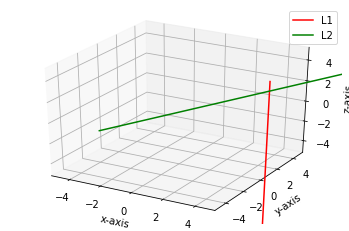
\includegraphics[width=\columnwidth]{download.png}
\caption{lines perpendicular to each other}
\label{Plot of the line}
\end{figure}
\end{document}



